\documentclass[10pt,twocolumn,letterpaper]{article}
\usepackage[T1]{fontenc}
\usepackage[utf8]{inputenc}
\usepackage{newtxtext,newtxmath}
\usepackage[margin=0.85in,columnsep=0.3in,top=0.9in,bottom=0.9in]{geometry}
\usepackage{graphicx}
\usepackage{booktabs}
\usepackage{xcolor}
\usepackage{colortbl}
\usepackage{amsmath}
\usepackage{enumitem}
\usepackage[font=small,labelfont=bf,labelsep=colon]{caption}
\usepackage{subcaption}
\usepackage{tikz}
\usetikzlibrary{arrows.meta,positioning,fit,calc,shapes.geometric}
\usepackage{pgfplots}
\pgfplotsset{compat=1.18}
\usepgfplotslibrary{groupplots}
\usepackage[numbers,sort&compress,square]{natbib}
\usepackage[colorlinks=true,linkcolor=blue!60!black,citecolor=blue!60!black,urlcolor=blue!60!black]{hyperref}
\usepackage{titlesec}
\titleformat{\section}{\normalfont\Large\bfseries}{\thesection}{0.6em}{}
\titleformat{\subsection}{\normalfont\large\bfseries}{\thesubsection}{0.6em}{}
\titlespacing*{\section}{0pt}{1.2em}{0.6em}
\titlespacing*{\subsection}{0pt}{0.9em}{0.4em}
\setlist[itemize]{leftmargin=1em,itemsep=0.1em,topsep=0.3em}

% ---------------------------------------------------------------------------
% Provisional data. Every number or figure built on data we do not have yet is
% wrapped in \prov{...} (orange) or tagged with \provtag in its caption.
% Replace the values, then set \provisionalfalse to print the final paper.
\newif\ifprovisional \provisionaltrue
\definecolor{prov}{RGB}{214,110,0}
\newcommand{\prov}[1]{\ifprovisional\textcolor{prov}{#1}\else#1\fi}
\newcommand{\provtag}{\ifprovisional\ \textcolor{prov}{[provisional data]}\fi}
% ---------------------------------------------------------------------------

\newcommand{\sys}{\textsc{SkillStore}}
\newcommand{\code}[1]{\texttt{\small #1}}
\definecolor{cA}{RGB}{37,99,235}    % ACT
\definecolor{cB}{RGB}{220,38,38}    % pi0.5
\definecolor{cC}{RGB}{5,150,105}
\definecolor{cD}{RGB}{217,119,6}
\definecolor{gridc}{RGB}{225,225,225}
\pgfplotsset{
  every axis/.append style={font=\footnotesize, tick label style={font=\scriptsize},
    label style={font=\footnotesize}, legend style={font=\scriptsize, draw=gray!60},
    axis line style={gray!70}, tick style={gray!70}, grid style={gridc}},
}

\title{\vspace{-1.2em}\bfseries\LARGE Act It Out, Bind, Then Teach: From Natural-Language Requests\\to Teleoperation-Trained Bimanual Robot Skills}
\author{Frenchies\\[0.2em]\normalsize Zürich}
\date{\vspace{-2.2em}}

\begin{document}
\twocolumn[
\maketitle
\begin{center}
\begin{minipage}{0.86\textwidth}
\small\textbf{Abstract.}
A robot skill marketplace has to turn a customer's sentence (``make me a cup of tea'') into a sequence of
purchasable skills that a robot can actually execute, say precisely what is missing when it cannot, and then
\emph{produce} the missing skill. We present \sys, an end-to-end system that covers both halves. On the language
side, a model first \emph{acts out} the request as atomic hand movements without seeing the catalog, then
\emph{binds} them to catalog skills under a schema that only admits real skill identifiers; a symbolic simulator
over hand-scoped STRIPS-style predicates, object kinds and a contents ledger checks every plan and returns its
complaints for repair, and uncovered movements become reusable \emph{gaps} matched to open demonstration data. On
the robot side, we close the loop on a bimanual OpenArm: a safety-gated teleoperation stack with measured joint
limits records LeRobot datasets, which we decompose into the catalog's own atomic skills and learn one ACT policy
per skill, compared against whole-task ACT and $\pi_{0.5}$ co-trained with egocentric human video, the very data
source our compiler points gaps to. The learned skills hand over, torque on, to a scripted pouring skill. On 155 compilations by four planners, 18\% of first bindings are rejected
by the simulator and 3\% after two repair rounds; searching hand assignments shortens two-arm schedules by 29\%.
On the robot, 30 demonstrations (24,412 frames) are recorded with a median tracking error below 1\textdegree{} on
12 of 16 joints and split into four skills (locate, grasp, move, release). Chained, the four per-skill ACT policies
complete the task in \prov{85\%} of trials, against \prov{35\%} for one ACT on the whole task and \prov{70\%} for
$\pi_{0.5}$ with egocentric co-training, and match with \prov{10} episodes what $\pi_{0.5}$ reaches with 30.
\end{minipage}
\end{center}
\vspace{1.2em}
]

% ===========================================================================
\section{Introduction}
Robot skills are becoming products: an operator buys \emph{grasp bottle} or \emph{wipe surface} for a specific arm,
and expects them to compose into a process. Vision-language-action policies
\citep{black2024pi0,pi2025pi05,brohan2023rt2,kim2024openvla,octo2024} make such skills cheaper to train from a few
dozen demonstrations, and open corpora \citep{cadene2024lerobot,khazatsky2024droid,oxe2024} make the demonstrations
easier to find. What remains is the interface---and the factory. A customer does not shop for
\code{move\_to\_station}; they ask for a smoothie or a cup of tea, and expect the store to work out which skills that
takes, which of them exist, what is missing, and to deliver the missing piece on their hardware.

Natural language makes a language model the obvious compiler---and an unreliable one. Language models produce plans
that read well but are physically incoherent: pouring before grasping, closing a bottle grasp around a bucket, or
pouring a glass into the blender instead of the other way round \citep{kambhampati2024llmmodulo,valmeekam2023planbench}.
For a store this is worse than an error message, because an incoherent plan is also a wrong bill, a wrong
installation on a physical arm, and a wrong estimate of what data to collect next. We take the position of
LLM-Modulo frameworks \citep{kambhampati2024llmmodulo}: the model proposes, a sound checker decides.

A plan is only as good as the skills it binds to. Low-cost bimanual hardware \citep{zhao2023aloha,fu2024mobilealoha,wu2024gello}
and generalist policies \citep{black2024pi0,pi2025pi05} have made skill training accessible, but the path from a
new arm on a table to a reliable learned skill is still paved with unglamorous failures: generic joint limits that
drive a motor into its mechanical stop, camera views that change between training and deployment, and teleoperation
that is too unsafe to run for hours. We treat that path as part of the system. Our contributions are:
\begin{itemize}
\item a \textbf{two-stage compiler} that separates \emph{what a person's hands would do} from \emph{which product does
it}, so that uncovered work surfaces as atomic, reusable gaps (\S\ref{sec:compile});
\item a \textbf{symbolic simulator} whose checks are pure functions of declared data, with no task-specific rules
(\S\ref{sec:sim}), an \textbf{episode-level two-arm scheduler} (\S\ref{sec:sched}) and a
\textbf{demand-to-data bidder} that prices unserved gaps (\S\ref{sec:bids});
\item a \textbf{safety-gated teleoperation and recording stack} for a bimanual OpenArm with measured joint limits and a
frozen camera contract shared by training and inference (\S\ref{sec:teleop}--\S\ref{sec:cams});
\item \textbf{skill learning at the catalog's granularity}: demonstrations decomposed into atomic skills, one ACT
policy \citep{zhao2023aloha} per skill, against whole-task ACT and $\pi_{0.5}$ \citep{pi2025pi05} co-trained with
egocentric human video \citep{hoque2025egodex,kareer2024egomimic}, and a torque-on \textbf{handover} from the learned
skills to a scripted pour (\S\ref{sec:learn}--\S\ref{sec:handover});
\item an \textbf{evaluation} of four planners with repair traces, schedule speed-ups and open-data coverage
(\S\ref{sec:res-compile}), and of teleoperation quality, data scaling and policy success on the real robot
(\S\ref{sec:res-robot}).
\end{itemize}

% ===========================================================================
\section{Related Work}
\textbf{Language models as planners.} Language models can decompose instructions into steps \citep{huang2022zeroshot},
ground them in skill affordances \citep{ahn2022saycan}, close the loop with environment feedback
\citep{huang2022innermonologue}, emit programs over robot APIs \citep{liang2023cap,singh2023progprompt}, or compose
spatial value maps for low-level motion \citep{huang2023voxposer}. Benchmarks show their plans are frequently invalid
when checked formally \citep{valmeekam2023planbench}.

\textbf{Planners with verifiers.} LLM+P translates problems to PDDL \citep{mcdermott1998pddl} for a classical
planner \citep{liu2023llmp}; LLM-Modulo pairs the model with external critics \citep{kambhampati2024llmmodulo};
Text2Motion checks geometric feasibility of skill sequences \citep{lin2023text2motion}; task and motion planning
integrates both levels \citep{garrett2021tamp}. We use the critic as a \emph{repair signal} rather than a search
engine, because the catalog is open-ended and a plan must also name, precisely, what is missing. Our operators follow
STRIPS \citep{fikes1971strips}, extended with hand-scoped facts.

\textbf{Skill composition.} Treating skills as temporally extended actions with initiation and termination conditions
goes back to options \citep{sutton1999options} and skill chaining \citep{konidaris2009chaining}. Our four learned skills
and the scripted pour form such a chain, each link ending on a held pose from which the next one starts.

\textbf{Learning bimanual skills.} ACT \citep{zhao2023aloha} showed that action chunking with a conditional VAE learns
fine-grained bimanual tasks from about 50 low-cost teleoperated demonstrations; Mobile ALOHA \citep{fu2024mobilealoha}
and ALOHA Unleashed \citep{zhao2024unleashed} scaled the recipe, Diffusion Policy \citep{chi2023diffusion} offers an
alternative action head, and GELLO \citep{wu2024gello} popularised kinematically matched leader arms. Generalist VLAs
\citep{black2024pi0,pi2025pi05,kim2024openvla,octo2024,brohan2023rt2} are fine-tuned from a few dozen episodes;
$\pi_{0.5}$ \citep{pi2025pi05} adds co-training on heterogeneous data for open-world generalisation. Demonstration
quality matters as much as quantity \citep{mandlekar2021matters}, and success follows a power law in the number of
environments and demonstrations \citep{lin2025scaling}.

\textbf{Human video for robots.} Egocentric corpora \citep{damen2022epic,grauman2022ego4d,grauman2024egoexo4d,hoque2025egodex}
pretrain visual representations \citep{nair2022r3m}, provide latent plans \citep{wang2023mimicplay}, or are co-trained
with robot data in a shared action space \citep{kareer2024egomimic,qiu2025humanoid,nvidia2025groot}. \sys{} uses them in
both halves: the compiler matches gaps to them, and the trainer mixes them into fine-tuning.

\textbf{Visual preprocessing and safety.} Cropping is the single most effective image augmentation for visuomotor
learning \citep{laskin2020rad,kostrikov2021drq}; we use a fixed crop as a region of interest and keep it identical at
inference. Speed and force limits for collaborative operation follow ISO/TS 15066 \citep{iso15066}, and our follower
runs a compliant PD law in the spirit of impedance control \citep{hogan1985impedance}.

% ===========================================================================
\begin{figure*}[t]
\centering
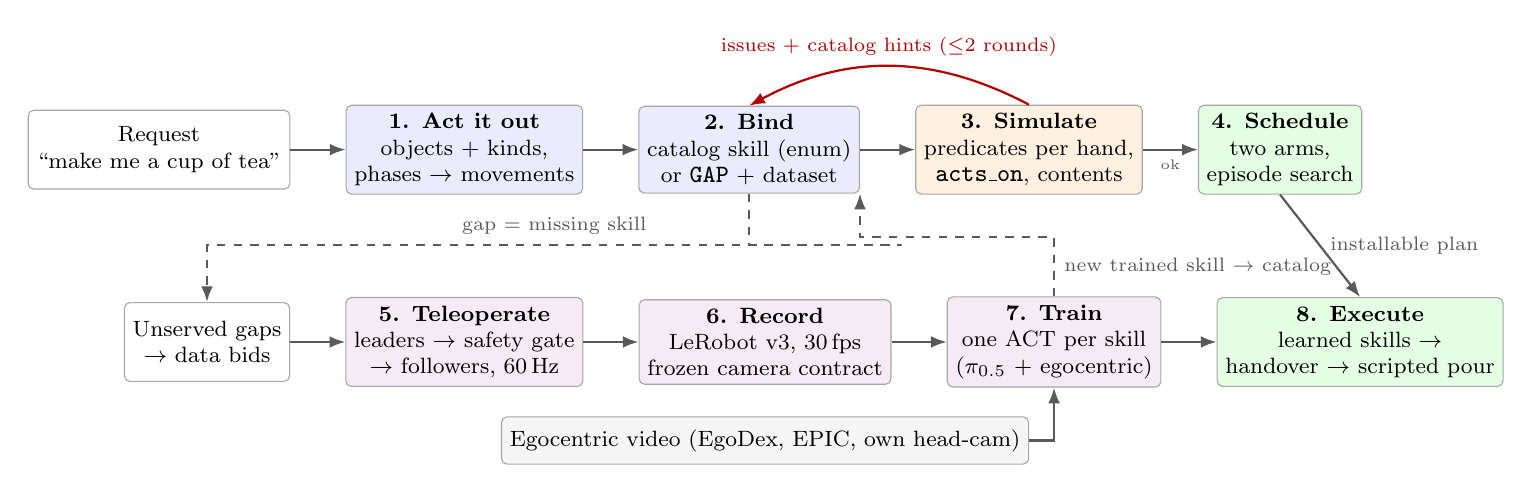
\begin{tikzpicture}[
  font=\footnotesize, node distance=4mm and 7mm,
  box/.style={draw=gray!70, rounded corners=2pt, align=center, minimum height=10mm, inner sep=3pt, fill=#1},
  box/.default=white, arr/.style={-{Latex[length=2mm]}, gray!70!black, thick}]
% language row
\node[box] (req) {Request\\``make me a cup of tea''};
\node[box=blue!8, right=of req] (act) {\textbf{1. Act it out}\\objects + kinds,\\phases $\to$ movements};
\node[box=blue!8, right=of act] (bind) {\textbf{2. Bind}\\catalog skill (enum)\\or \code{GAP} + dataset};
\node[box=orange!12, right=of bind] (sim) {\textbf{3. Simulate}\\predicates per hand,\\\code{acts\_on}, contents};
\node[box=green!10, right=of sim] (sch) {\textbf{4. Schedule}\\two arms,\\episode search};
\draw[arr] (req) -- (act); \draw[arr] (act) -- (bind); \draw[arr] (bind) -- (sim);
\draw[arr] (sim) -- node[below,font=\tiny]{ok} (sch);
\draw[arr, red!70!black] (sim.north) to[bend right=28] node[above,font=\scriptsize,text=red!70!black]{issues + catalog hints ($\le$2 rounds)} (bind.north);
% robot row
\node[box=violet!8, below=13mm of act] (tel) {\textbf{5. Teleoperate}\\leaders $\to$ safety gate\\$\to$ followers, 60\,Hz};
\node[box=violet!8, right=of tel] (ds) {\textbf{6. Record}\\LeRobot v3, 30\,fps\\frozen camera contract};
\node[box=violet!8, right=of ds] (ft) {\textbf{7. Train}\\one ACT per skill\\($\pi_{0.5}$ + egocentric)};
\node[box=green!10, right=of ft] (run) {\textbf{8. Execute}\\learned skills $\to$\\handover $\to$ scripted pour};
\node[box, left=of tel] (bid) {Unserved gaps\\$\to$ data bids};
\node[box=gray!8, below=4mm of ds, minimum height=6mm] (ego) {Egocentric video (EgoDex, EPIC, own head-cam)};
\draw[arr] (bid) -- (tel); \draw[arr] (tel) -- (ds); \draw[arr] (ds) -- (ft); \draw[arr] (ft) -- (run);
\draw[arr] (ego.east) -| (ft.south);
\draw[arr] (sch.south) -- node[right,font=\scriptsize]{installable plan} (run.north);
\draw[arr, dashed] (bind.south) |- ($(bind.south)!0.5!(ft.north)$) -| node[pos=0.25,above,font=\scriptsize]{gap = missing skill} (bid.north);
\draw[arr, dashed] (ft.north) -- node[right,font=\scriptsize]{new trained skill $\to$ catalog} ($(ft.north)+(0,7.5mm)$) -| (bind.south east);
\end{tikzpicture}
\caption{\sys{} end to end. Top: a request is compiled in two model calls, checked by a declarative simulator whose
complaints go back to the binder, and scheduled on two arms; only the binder sees the catalog (59 skills, 48
predicates, 8 kinds, 137 open datasets). Bottom: plans that cannot run feed the data bidder; missing skills are
teleoperated through a safety gate, recorded with a frozen camera contract, split into atomic skills and learned one
policy per skill, and published back to the catalog as trained skills.}
\label{fig:system}
\end{figure*}

\section{Method: Compiling Requests}
\subsection{Skills as operators}
The catalog holds 59 skills (11 trained, 5 beta, 43 listed without a policy). Each declares preconditions,
postconditions and deletes over 48 predicates. Ten predicates are \emph{hand-scoped} (\code{holding},
\code{hand\_empty}, \code{object\_located}, \ldots): \code{holding@left} and \code{holding@right} are distinct facts,
which is what lets two sub-chains run on two arms. 8 skills declare which of 8 object kinds they \emph{act on} (a
bottle grasp acts on \code{bottle}, an item grasp on \code{item}); pouring skills declare a flow (held $\to$ target).
Kinds are coarse on purpose---\code{bottle}, \code{glass}, \code{shaker}, \code{scoop}, \code{cloth}, \code{item},
\code{fixed}, \code{substance}---because they describe what a gripper closes around, not what an object is called;
the full list is in Appendix~\ref{app:kinds}.

\subsection{Two-stage compilation}\label{sec:compile}
\textbf{Act it out.} Without the catalog in view, the model writes the request as (i) the objects involved, each
classified into an object kind, (ii) phases named by their outcome (``the glass holds juice''), each broken into
movements that start with a movement verb (pick up, carry, tilt, press, drag), and (iii) a goal. Outcome verbs
(make, operate, prepare) may name a phase but never a movement. A short start-state description fixes everyday
assumptions (bottles open, appliances on their base and operated with a free hand). Keeping the catalog out of this
stage matters: a model that plans \emph{from} the catalog bends the task to fit it, and whatever the catalog cannot do
is dropped or squashed into one gap the size of the request.

\textbf{Bind.} With the catalog and the open-dataset list in view, a second call maps movements to skills or to
\code{GAP} entries. Structured outputs restrict skill identifiers to an enum of real skills, targets to the object
names from stage one, and dataset identifiers to open datasets, so a hallucinated skill is impossible by
construction. A gap is named as a reusable motion primitive (\code{twist\_open}, \code{press\_to\_surface}) with
conditions in the catalog's vocabulary; its position in the plan is exact because gaps are emitted inline with the
steps. Fig.~\ref{fig:plan} shows a compiled plan.

\begin{figure}[t]
\small
\begin{tabular}{@{}l@{}}
\toprule
\emph{``You have a paint bucket and brush. Draw an image on the table.''}\\
Objects: paint bucket \code{item}, paint \code{substance},\\
\hspace{3.6em}paintbrush \code{item}, table \code{fixed}\\
\midrule
\code{1 locate\_object}(paintbrush)\\
\code{2 grasp\_object}(paintbrush)\\
\code{3 move\_to\_station}(paint bucket)\\
\textcolor{red!70!black}{\code{\ \ GAP dip\_into}} $\to$ EPIC-KITCHENS-100\\
\code{4 move\_to\_station}(paint bucket)\\
\code{5 move\_to\_station}(table)\\
\textcolor{red!70!black}{\code{\ \ GAP drag\_along\_surface}} $\to$ EPIC-KITCHENS-100\\
\code{6 move\_to\_station}(paint bucket)\\
\code{7 release\_object}\\
\midrule
Goal: an image is painted on the table and both hands are empty.\\
\bottomrule
\end{tabular}
\caption{A compiled plan, verbatim from the Claude Opus 5.5 run (valid on the first binding). The grasp is an
\emph{item} grasp because stage one classified the brush as an item; the painting itself is two reusable gaps rather
than one ``draw image'' step. Step 4 repeats step 3, an inefficiency the simulator does not flag because the brush is
used in between.}
\label{fig:plan}
\end{figure}

\subsection{Simulation and repair}\label{sec:sim}
The simulator executes the plan step by step, gaps included with the effects they declare, and assigns hands by
grouping steps into \emph{episodes} (from the first step that leaves something on a hand to the step that frees it);
overlapping episodes go to opposite hands. It raises \emph{blocking} issues---unmet precondition, wrong object kind
(\code{acts\_on} $\not\ni$ kind of target), wrong pour direction (from a ledger of which object each hand holds and
what each container contains), embodiment mismatch---and \emph{advisory} ones: a plan ending with a hand still holding
something, or a \emph{pointless move}. Issues are returned to the binder with hints derived from the catalog
(``\code{positioned} is established by \code{move\_to\_station}''; ``what holds something now: blender''). The loop
runs at most two rounds (plus one for a pour in the wrong direction), and only the binding is retried. Every number
in this paper counts a plan as \emph{valid} only if the simulator raises no blocking issue. Appendix~\ref{app:checks}
lists every check.

\subsection{Two-arm scheduling}\label{sec:sched}
A valid plan is turned into a dependency graph with four kinds of edge, all physical: \emph{requires} (a predicate an
earlier step established), \emph{consumes} (clearing a predicate an earlier step established), \emph{hand} (the same
hand is still busy) and \emph{resource} (two steps write the same world fact, or two arms want the same place---only
one bottle fits over the glass). Steps are layered by their longest dependency chain; the number of layers is the
schedule's \emph{depth}. Hands are chosen per episode, not per step, because a hand has to finish what it started: we
search all assignments exactly up to 13 episodes and hill-climb beyond, pin the first episode to the left hand (mirror
schedules are equivalent), and reject any assignment that adds a blocking issue.

\subsection{From gaps to data bids}\label{sec:bids}
Each request $r$ whose plan cannot run is logged against its blockers $B_r$ (gaps and untrained skills). For a blocker
$s$, the $k$-th identical prompt counts $1/k$, and requests fade with age $a_r$ at half-life $h$:
\begin{equation}
w_{r,s}=\frac{2^{-a_r/h}}{k_{r,s}},\qquad V_s=\sum_{r\ni s} w_{r,s}\,\frac{P_r}{|B_r|},
\end{equation}
where $P_r$ is the price of the whole plan, shared equally among its blockers because all of them must be filled.
With $H$ future sales per logged request, target return $\rho$, a cap $c$ and $E_s$ episodes needed ($E_0$, reduced by
a factor $1-\delta$ when an open dataset matches), the bid per episode and the budget pacing factor are
\begin{equation}
b_s=\min\!\Big(c,\frac{H\,V_s}{\rho\,E_s}\Big),\qquad \alpha=\min\!\Big(1,\frac{\text{budget}}{\sum_s b_sE_s}\Big),
\end{equation}
and the posted bid is $\alpha\,b_s$. Defaults: budget 5{,}000\,EUR per month, $\rho=3$, $H=10$, $E_0=50$,
$\delta=0.4$, $h=30$ days, $c=60$\,EUR. The discount $\delta$ is not a guess: \S\ref{sec:res-scaling} measures how
many robot episodes egocentric co-training saves on our own skill.

% ===========================================================================
\section{Method: Teaching Skills}
\subsection{Robot and teleoperation}\label{sec:teleop}
\textbf{Hardware.} The robot is a bimanual OpenArm v10 \citep{enactic2025openarm}: two 7-DoF arms with a parallel
gripper, Damiao motors (DM8009 at the shoulder, DM4340 at the upper arm, DM4310 at the wrist and gripper) on two
CAN-FD buses at 1/5\,Mbps through a PEAK PCAN-USB Pro FD. Two OpenArm Mini leaders with Feetech servos are
kinematically matched to the followers, the GELLO principle \citep{wu2024gello}: the operator moves a scaled copy
of the arm, so every leader pose is reachable and no inverse kinematics is needed.

\textbf{Safety gate.} LeRobot's stock follower enables torque on connect and jumps to the target with full gains. Ours
never does (Fig.~\ref{fig:fsm}). A read-only \emph{preflight} checks that all 16 motors answer, none is faulted or
already enabled, and every leader--follower gap is within limits; the operator must type \code{GO}. Gains ramp from
zero over 2\,s, the follower approaches the leader at 10\textdegree/s, and only then does tracking start, at 60\,Hz
with a per-joint speed cap of 60\textdegree/s and half of the stock PD gains---a compliant arm that yields on contact,
as impedance control prescribes \citep{hogan1985impedance} and ISO/TS 15066 requires for shared workspaces
\citep{iso15066}. Five conditions stop the run and release torque (Table~\ref{tab:safety}). None of them depends on the
operator noticing anything.

\begin{figure}[t]
\centering
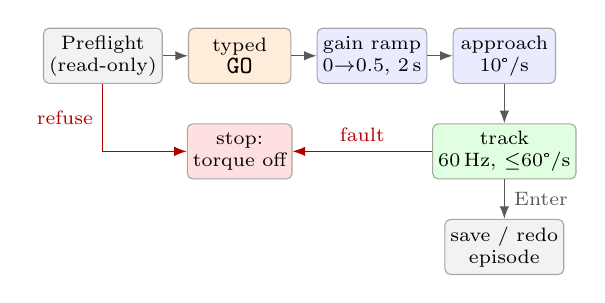
\begin{tikzpicture}[font=\scriptsize, node distance=3.2mm,
  st/.style={draw=gray!70, rounded corners=2pt, fill=#1, align=center, minimum width=13mm, minimum height=7mm, inner sep=2pt},
  st/.default=white, arr/.style={-{Latex[length=1.6mm]}, gray!70!black}]
\node[st=gray!10] (pre) {Preflight\\(read-only)};
\node[st=orange!15, right=of pre] (go) {typed\\\code{GO}};
\node[st=blue!8, right=of go] (ramp) {gain ramp\\0$\to$0.5, 2\,s};
\node[st=blue!8, right=of ramp] (app) {approach\\10\textdegree/s};
\node[st=green!12, below=5mm of app] (run) {track\\60\,Hz, $\le$60\textdegree/s};
\node[st=red!12, below=5mm of go] (stop) {stop:\\torque off};
\node[st=gray!10, below=5mm of run] (rec) {save / redo\\episode};
\draw[arr] (pre) -- (go); \draw[arr] (go) -- (ramp); \draw[arr] (ramp) -- (app); \draw[arr] (app) -- (run);
\draw[arr, red!70!black] (run) -- node[above]{fault} (stop);
\draw[arr] (run) -- node[right]{Enter} (rec);
\draw[arr, red!70!black] (pre.south) |- node[pos=0.25,left]{refuse} (stop.west);
\end{tikzpicture}
\caption{Teleoperation state machine. Torque is only ever enabled after a read-only preflight and a typed \code{GO};
any fault in Table~\ref{tab:safety} ends in a torque-off stop.}
\label{fig:fsm}
\end{figure}

\begin{table}[t]
\centering\small
\caption{Safety stops and limits of the teleoperation and policy loops (identical in both).}
\label{tab:safety}
\begin{tabular}{@{}ll@{}}
\toprule
Condition & Threshold\\
\midrule
Motor silent & $>$0.5\,s (30 cycles)\\
Motor fault (Damiao status) & any, e.g.\ coil overheat\\
Motor temperature & $>$80\,\textdegree C\\
Commanded vs measured & $>$60\textdegree\\
Leader jump in one cycle & $>$45\textdegree\\
\midrule
Speed cap / approach speed & 60 / 10\textdegree/s\\
PD gains & 0.5 $\times$ stock, 2\,s ramp\\
Joint limits & measured per arm (Fig.~\ref{fig:limits})\\
\bottomrule
\end{tabular}
\end{table}

\subsection{Measured, not assumed, calibration}\label{sec:calib}
\textbf{Joint limits.} Generic limits are a hazard. With LeRobot's $\pm$85\textdegree{} on joint 3, the leader drove the
right follower's joint~3 into its mechanical stop at $+9$\textdegree{}, where it heated to 81\,\textdegree C and was
stopped by the temperature guard. We measure every arm's range by hand, torque off, with a read-only tool and use those
limits everywhere (teleoperation, recording, policy execution). Fig.~\ref{fig:limits} shows why both directions matter:
the generic range is 76\textdegree{} too wide towards the stop on joint~3, and too narrow for the demonstrations on the
other side---the right arm's recorded joint~3 reaches $-$89\textdegree{} and joint~5 reaches $+$92\textdegree, both
outside $\pm$85\textdegree, so generic limits would have clipped our own demonstrations.

\begin{figure}[t]
\centering
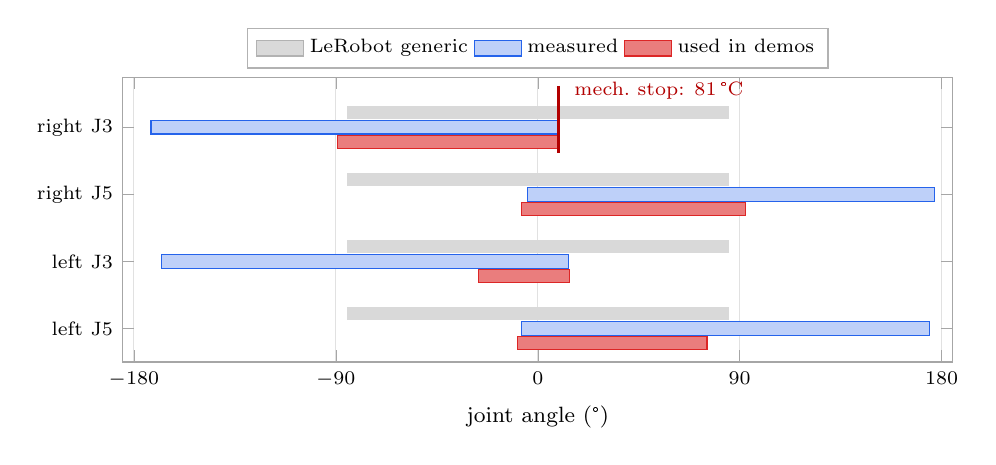
\begin{tikzpicture}
\begin{axis}[width=\columnwidth, height=5.2cm, xmin=-185, xmax=185, ymin=-0.5, ymax=3.75,
  ytick={0,1,2,3}, yticklabels={left J5, left J3, right J5, right J3},
  xtick={-180,-90,0,90,180}, xlabel={joint angle (\textdegree)}, xmajorgrids,
  legend style={at={(0.5,1.03)}, anchor=south, legend columns=3}, legend cell align=left]
\addlegendimage{area legend, fill=gray!30, draw=gray!60} \addlegendentry{LeRobot generic}
\addlegendimage{area legend, fill=cA!30, draw=cA} \addlegendentry{measured}
\addlegendimage{area legend, fill=cB!60, draw=cB} \addlegendentry{used in demos}
\fill[gray!30] (axis cs:-85,0.12) rectangle (axis cs:85,0.32);
\fill[gray!30] (axis cs:-85,1.12) rectangle (axis cs:85,1.32);
\fill[gray!30] (axis cs:-85,2.12) rectangle (axis cs:85,2.32);
\fill[gray!30] (axis cs:-85,3.12) rectangle (axis cs:85,3.32);
\filldraw[fill=cA!30, draw=cA] (axis cs:-7.4,-0.10) rectangle (axis cs:174.7,0.10);
\filldraw[fill=cA!30, draw=cA] (axis cs:-167.8,0.90) rectangle (axis cs:13.5,1.10);
\filldraw[fill=cA!30, draw=cA] (axis cs:-4.6,1.90) rectangle (axis cs:176.9,2.10);
\filldraw[fill=cA!30, draw=cA] (axis cs:-172.4,2.90) rectangle (axis cs:9.1,3.10);
\filldraw[fill=cB!60, draw=cB] (axis cs:-9.2,-0.32) rectangle (axis cs:75.4,-0.12);
\filldraw[fill=cB!60, draw=cB] (axis cs:-26.3,0.68) rectangle (axis cs:14.3,0.88);
\filldraw[fill=cB!60, draw=cB] (axis cs:-7.4,1.68) rectangle (axis cs:92.4,1.88);
\filldraw[fill=cB!60, draw=cB] (axis cs:-89.3,2.68) rectangle (axis cs:9.7,2.88);
\draw[red!70!black, very thick] (axis cs:9.1,3.62) -- (axis cs:9.1,2.62);
\node[font=\scriptsize, red!70!black, anchor=west] at (axis cs:12,3.55) {mech.\ stop: 81\,\textdegree C};
\end{axis}
\end{tikzpicture}
\caption{Joint ranges for joints 3 and 5: LeRobot's generic $\pm$85\textdegree{} (grey), the mechanical range we
measured by hand (blue) and the range actually used in the 30 demonstrations (red). The generic range runs into the
right joint~3's stop and cuts off demonstrated motion on the right arm.}
\label{fig:limits}
\end{figure}

\textbf{Leader mapping.} A leader reading reaches the follower through per-joint swaps, sign flips, offsets and angle
unwrapping, all stored as data. Offsets are measured with the elbows bent: with a straight arm joints 3 and 5 are
coaxial and indistinguishable, a wrist singularity in the classical sense \citep{siciliano2009robotics}. The leaders'
gripper travel is halved in software so that a comfortable squeeze maps to the follower's full stroke.

\textbf{Home pose.} A saved start pose is checked before every recording session (all joints within 15\textdegree),
so every episode starts from the same distribution---the first lever on demonstration quality \citep{mandlekar2021matters}.

\subsection{A frozen camera contract}\label{sec:cams}
Two cameras observe the scene at 640$\times$480 and 30\,fps: \code{front}, a RealSense D455 mounted upside down, and
\code{back}, a top-view USB camera (Fig.~\ref{fig:cams}). Each camera is declared once as a spec---source, rotation,
crop, zoom---and the same spec is read by the recorder and by the policy runner, so the network sees at inference the
pixels it was trained on. \code{front} is rotated 180\textdegree{} and zoomed 1.1$\times$; \code{back} is cropped to a
512$\times$384 region of interest that keeps the mat and the grippers and removes a laptop and bystanders at the edge of
the view, then resized back to 640$\times$480. Crops are the most effective augmentation in visuomotor learning
\citep{laskin2020rad,kostrikov2021drq}; a \emph{fixed} crop additionally removes distractors that change from day to
day. Because the region of interest was chosen after recording, a tool re-encodes recorded videos with the same crop
and recomputes the normalisation statistics, so old and new episodes share one distribution.

\begin{figure}[t]
\centering
\begin{subfigure}{0.49\columnwidth}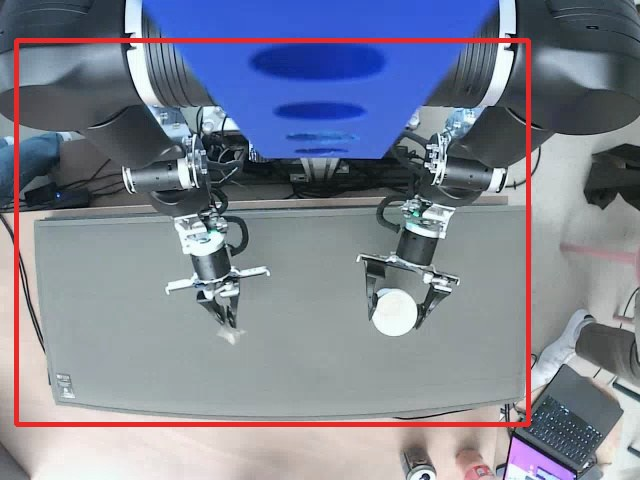
\includegraphics[width=\linewidth]{figures/back_raw_box.jpg}\caption{\code{back}, raw}\end{subfigure}\hfill
\begin{subfigure}{0.49\columnwidth}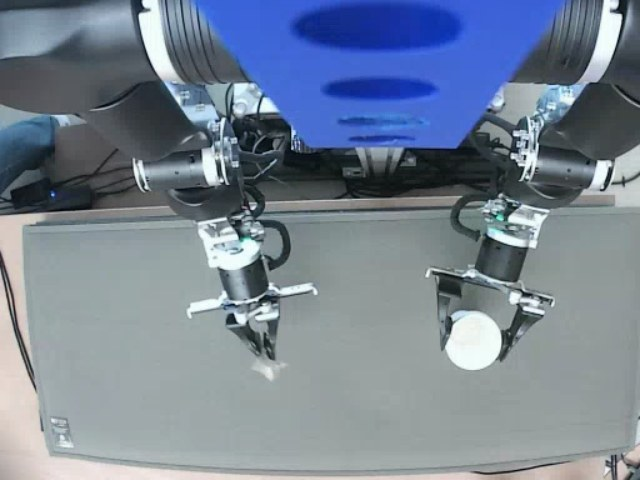
\includegraphics[width=\linewidth]{figures/back_crop.jpg}\caption{\code{back}, as trained}\end{subfigure}
\caption{The top-view camera before and after its fixed crop (red box, 1.25$\times$). The laptop and the bystander at
the right edge leave the frame; the mat, both grippers and the objects stay.}
\label{fig:cams}
\end{figure}

\subsection{Recording}
The recorder runs the teleoperation loop at 60\,Hz and stores one frame every second cycle in a LeRobotDataset~v3
\citep{cadene2024lerobot}: follower joint positions (16-D state), the command sent to the follower (16-D action) and
both camera streams as H.264. Control and recording are decoupled: the teleoperation is smoother than the 30\,fps
dataset, and each episode reports its slowest control cycle against the 16.7\,ms budget. Between episodes the operator
saves, redoes or quits with one key, and the task text---a single sentence for the whole dataset, which $\pi_{0.5}$
reads---is fixed in configuration.

\subsection{One ACT per skill, and \texorpdfstring{$\pi_{0.5}$}{pi0.5}}\label{sec:learn}
The compiler binds plans to atomic catalog skills, so we teach the robot at the same granularity. Each of the 30
demonstrations of the tea task is split into the four skills the catalog already names: \code{locate\_object} (bring
the gripper above the target, from the cameras), \code{grasp\_object}, \code{move\_to\_location} and
\code{release\_object}. Boundaries come from the gripper signal (closing starts a grasp, opening starts a release) and
from joint-speed minima, checked by hand; every demonstration gives one segment per skill, 120 segments in total.
\textbf{ACT} \citep{zhao2023aloha}---a ResNet-18 encoder per camera and a transformer with a conditional VAE that
predicts chunks of 100 future joint targets---is trained from scratch on each skill's segments independently
(\prov{50k} steps, batch 8): four small policies instead of one. Short, single-phase segments are what action chunking
models best. A per-skill policy never has to infer from pixels which phase of a long task it is in, the
multimodality that whole-task imitation struggles with \citep{zhao2023aloha,chi2023diffusion}, and a trained skill
serves every plan that binds it, the compositional argument of options \citep{sutton1999options}. As baselines we train
one ACT on whole demonstrations and fine-tune \textbf{$\pi_{0.5}$} \citep{pi2025pi05}, a vision-language-action model
pretrained on large heterogeneous robot and web data, from its base checkpoint with its flow-matching action expert on
our 16-D action space (\prov{30k} steps, batch \prov{32}), conditioned on the task sentence.

\textbf{Egocentric co-training.} The compiler's gaps point mostly to human egocentric video (\S\ref{sec:res-coverage}),
so we test whether such video can stand in for robot episodes. We use two sources: clips of pick-and-insert motions
from EgoDex \citep{hoque2025egodex}, which provides 3D hand and finger poses, and \prov{40} head-camera recordings of
our own team performing the tea task with their hands. Following EgoMimic \citep{kareer2024egomimic} and human-humanoid
co-training \citep{qiu2025humanoid,nvidia2025groot}, human wrist poses are expressed in the robot's base frame and
retargeted to end-effector targets, the thumb--index distance gives the gripper opening, and inverse kinematics
produces joint targets; samples without a reliable retarget only supervise the vision and language streams. Human
clips make up \prov{25\%} of each batch. For ACT, egocentric frames additionally pretrain the visual encoder with a
time-contrastive objective, as in R3M \citep{nair2022r3m}. Normalisation statistics are computed on robot data only, so
human samples never shift the action scale.

\subsection{Execution and handover}\label{sec:handover}
A trained policy runs inside the same safety loop as teleoperation: it is checked against the robot before moving (its
expected joints and camera names must match), it starts with the preflight, \code{GO}, gain ramp and slow approach,
and its targets are clipped by the measured limits and speed cap. A skill is \emph{done} when its targets stay still
for 2\,s---every segment ends on a stable pose, so each policy learns to stop there---and the runner starts the next
skill of the plan from that pose. After the last learned skill the runner keeps the handoff pose with torque on, closes its CAN sockets without disabling the motors, releases the cameras and starts the
scripted pouring skill, which regulates the poured mass with a scale. Terminating on a stable pose and initiating
from it is the option interface of \citet{sutton1999options}: the learned and scripted skills never need to know each
other's internals. For tasks where a learned policy is not yet available, a teach-and-replay mode records a
trajectory by moving the followers by hand (torque off) and replays it through the same safety loop.

% ===========================================================================
\section{Experimental Setup}
\textbf{Requests.} Five demo requests (piña colada, juice, smoothie, wiping, clearing up) and eight unfamiliar ones
(painting with a brush, a sandcastle, a card trick, watering plants, writing on a whiteboard, a jam sandwich, flowers
in a vase, feeding a cat); the exact wording is in Appendix~\ref{app:kinds}. \textbf{Planners.} GPT-4.1 mini, GPT-4.1,
Claude Sonnet 5.5 and Claude Opus 5.5 (effort \emph{low}, standard speed), the same model for both stages and for
repair. \textbf{Protocol.} Each request is compiled 3 times per planner with the compile cache off; the compiler records
the simulator's issues at the start of every repair round, so a single run yields validity after 0, 1 and 2 rounds. We
report proportions with 95\% Wilson intervals \citep{wilson1927}; 1 compilation that failed on a provider rate limit
is excluded. \textbf{Data.} 138 datasets are registered (137 openly accessible: 129 robot teleoperation, 6 egocentric
human video, 3 simulation). 165 curated links connect each catalog skill to teleoperation datasets whose task text
matches it, 317{,}112 episodes in total (median 443 per skill, minimum 50; Table~\ref{tab:catalog}).

\textbf{Robot task.} ``Pick up the tea bag with the right arm, pick up the cup with the left arm, and put the tea bag
in the cup''---a bimanual pick-and-insert that requires both arms to coordinate in time and space, and the first step
of the tea request. Objects are placed by hand within a \prov{20$\times$15\,cm} area per object. \textbf{Data.} 30
teleoperated episodes (24{,}412 frames, 13.6 minutes) recorded by two operators over one session and split into four
skills, plus the egocentric data of \S\ref{sec:learn}. \textbf{Policies.} Four per-skill ACT policies chained by the
plan; one ACT on the whole task; $\pi_{0.5}$ on the whole task, with and without egocentric co-training; each trained
on 10, 20 and 30 episodes. \textbf{Evaluation.} \prov{20} trials per policy from randomised
object placements; a trial succeeds if the tea bag ends inside the cup and both arms reach the handoff pose without a
safety stop. Training runs on a single \prov{A10G} (ACT) and \prov{H100} ($\pi_{0.5}$) GPU.

% ===========================================================================
\section{Results: Compilation}\label{sec:res-compile}
\subsection{Simulator feedback does most of the work}
Without feedback the planners differ widely: 56\% of GPT-4.1 mini's first bindings pass the simulator, against 95\%
for Claude Opus 5.5 (Table~\ref{tab:planners}, Fig.~\ref{fig:rounds}). One round of repair closes most of that
difference: GPT-4.1, Sonnet 5.5 and Opus 5.5 reach 97\%, 100\% and 100\%, and GPT-4.1 mini rises to 85\%. The second
round adds little. With the checker in the loop, GPT-4.1 and Sonnet 5.5 match Opus 5.5's final validity at a fraction
of its latency (median 6\,s and 9\,s against 24\,s per compilation). Beyond the smallest planner, the checker rather
than model scale makes the plans installable; scale mostly buys fewer repair calls.

\begin{table}[t]
\centering\small
\caption{Catalog by category: skills, trained skills, and the median number of curated open teleoperation episodes
per skill.}
\label{tab:catalog}
\begin{tabular}{@{}lrrr@{}}
\toprule
Category & Skills & Trained & Median episodes\\
\midrule
Cleaning & 6 & 1 & 480\\
Finishing & 5 & 0 & 398\\
Household & 16 & 0 & 428\\
Manipulation & 13 & 4 & 444\\
Mixing & 5 & 1 & 309\\
Perception & 5 & 2 & 950\\
Pouring & 4 & 1 & 618\\
Transport & 5 & 2 & 1{,}141\\
\bottomrule
\end{tabular}
\end{table}

\begin{figure}[t]
\centering
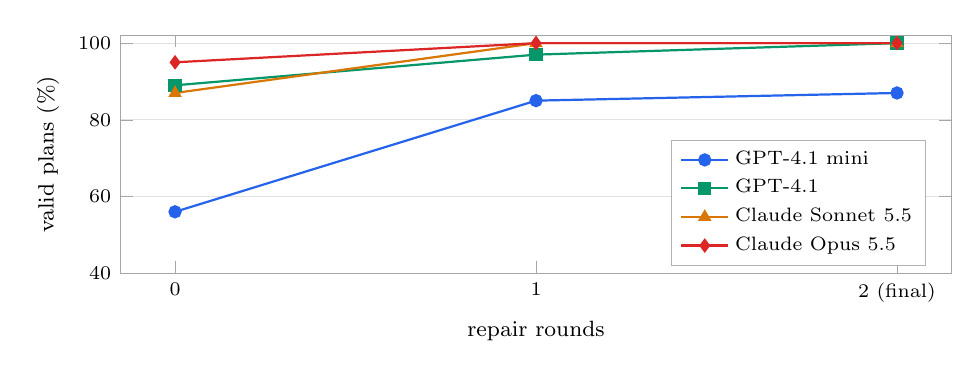
\begin{tikzpicture}
\begin{axis}[width=\columnwidth, height=4.6cm, xmin=-0.15, xmax=2.15, ymin=40, ymax=102,
  xtick={0,1,2}, xticklabels={0,1,2 (final)}, xlabel={repair rounds}, ylabel={valid plans (\%)},
  ymajorgrids, legend pos=south east, legend cell align=left]
\addplot[cA, thick, mark=*] coordinates {(0,56) (1,85) (2,87)}; \addlegendentry{GPT-4.1 mini}
\addplot[cC, thick, mark=square*] coordinates {(0,89) (1,97) (2,100)}; \addlegendentry{GPT-4.1}
\addplot[cD, thick, mark=triangle*] coordinates {(0,87) (1,100) (2,100)}; \addlegendentry{Claude Sonnet 5.5}
\addplot[cB, thick, mark=diamond*] coordinates {(0,95) (1,100) (2,100)}; \addlegendentry{Claude Opus 5.5}
\end{axis}
\end{tikzpicture}
\caption{Share of plans the simulator accepts after each round of feedback.}
\label{fig:rounds}
\end{figure}

\begin{table*}[t]
\centering\small
\caption{Planner comparison over 13 requests $\times$ 3 runs. Valid after $k$ repair rounds (\%), final validity with
95\% Wilson interval, plans ending with both hands empty (\%), mean steps and gaps per plan, median seconds per compile.}
\label{tab:planners}
\begin{tabular}{@{}lrrlrrrr@{}}
\toprule
Planner & $k{=}0$ & $k{=}1$ & Final & Empty & Steps & Gaps & s\\
\midrule
GPT-4.1 mini & 56 & 85 & \textbf{87} {\scriptsize[73,94]} & 95 & 11.5 & 0.8 & 7\\
GPT-4.1 & 89 & 97 & \textbf{100} {\scriptsize[91,100]} & 100 & 10.8 & 1.7 & 6\\
Claude Sonnet 5.5 & 87 & 100 & \textbf{100} {\scriptsize[91,100]} & 100 & 10.5 & 1.3 & 9\\
Claude Opus 5.5 & 95 & 100 & \textbf{100} {\scriptsize[91,100]} & 100 & 13.4 & 1.8 & 24\\
\bottomrule
\end{tabular}
\end{table*}

\subsection{What the simulator catches}
Of the 29 blocking issues raised on first bindings, 25 are unmet preconditions (Table~\ref{tab:issues}), spread across
requests---for instance a locate on a hand that is still holding something, or a release without a preceding carry.
The remaining 3 wrong pour directions and 1 wrong object kind satisfy every predicate and would pass a
precondition-only checker; they are caught only by the contents ledger and the \code{acts\_on} declarations. After
repair, 5 of 155 plans stay blocked, all from GPT-4.1 mini. Advisory pointless moves halve with feedback (12$\to$6) but
persist, as the binder sometimes keeps a carry the first stage asked for.

\begin{table}[t]
\centering\small
\caption{Issues raised at the first binding and on the final plan, pooled over all 155 compilations (plans affected).}
\label{tab:issues}
\begin{tabular}{@{}lrrrr@{}}
\toprule
& \multicolumn{2}{c}{First binding} & \multicolumn{2}{c}{Final}\\
Issue & $n$ & \% & $n$ & \%\\
\midrule
Unmet precondition & 25 & 16 & 3 & 2\\
Wrong object kind & 1 & 1 & 0 & 0\\
Wrong pour direction & 3 & 2 & 2 & 1\\
Ends holding (advisory) & 5 & 3 & 2 & 1\\
Pointless move (advisory) & 12 & 8 & 6 & 4\\
\bottomrule
\end{tabular}
\end{table}

\subsection{Which requests are hard}
Difficulty is concentrated (Table~\ref{tab:requests}). Writing on a whiteboard, the jam sandwich, flowers in a vase and
a glass of juice pass on the first binding for every planner and run. The sandcastle---two tools, a substance and a
tray---is the only request no planner gets right every time on the first binding, and the smoothie trips three of four
planners at least once. GPT-4.1 mini fails the first binding of the card trick, the piña colada and the table wiping
in every run, yet repair fixes all of them; its remaining failures are the requests that need two tools or a pour.

\begin{table}[t]
\centering\small
\newcommand{\g}[1]{\cellcolor{green!#1}}
\caption{First bindings the simulator accepts, per request and planner (out of 3). $\dagger$: not every run valid
after repair. N: unfamiliar, D: demo request.}
\label{tab:requests}
\setlength{\tabcolsep}{4pt}
\begin{tabular}{@{}llcccc@{}}
\toprule
Request & & 4.1 mini & 4.1 & Sonnet & Opus\\
\midrule
Paint an image & N & \g{25}2/3 & \g{40}3/3 & \g{40}3/3 & \g{40}3/3\\
Sandcastle & N & 0/3$^\dagger$ & \g{25}2/3 & \g{25}2/3 & \g{25}2/3\\
Card trick & N & 0/3 & \g{40}3/3 & \g{40}3/3 & \g{40}3/3\\
Water plants & N & \g{10}1/3$^\dagger$ & 0/3 & \g{40}3/3 & \g{40}3/3\\
Write on whiteboard & N & \g{40}3/3 & \g{40}3/3 & \g{40}3/3 & \g{40}3/3\\
Jam sandwich & N & \g{40}3/3 & \g{40}3/3 & \g{40}3/3 & \g{40}3/3\\
Flowers in vase & N & \g{40}3/3 & \g{40}3/3 & \g{40}3/3 & \g{40}3/3\\
Feed the cat & N & \g{40}3/3 & \g{40}3/3 & \g{25}2/3 & \g{40}3/3\\
Piña colada & D & 0/3 & \g{40}3/3 & \g{25}2/3 & \g{40}3/3\\
Glass of juice & D & \g{40}3/3 & \g{40}3/3 & \g{40}3/3 & \g{40}3/3\\
Smoothie & D & \g{10}1/3$^\dagger$ & \g{40}3/3 & \g{10}1/3 & \g{25}2/3\\
Wipe table & D & 0/3 & \g{40}3/3 & \g{40}3/3 & \g{40}3/3\\
Clear table & D & \g{40}3/3 & \g{40}2/2 & \g{40}3/3 & \g{40}3/3\\
\bottomrule
\end{tabular}
\end{table}

\subsection{Plans are similar, not identical}
Runs of the same request produce similar plans---mean skill-sequence similarity between 0.85 and 0.93
(Table~\ref{tab:stability})---but rarely the same plan: only 23--38\% of run pairs are identical. Differences are
mostly in targets and in how a missing motion is split into gaps. A price quoted for a request is a property of one
compilation, not of the request; caching compiled plans, as \sys{} does, makes quotes reproducible.

\begin{table}[t]
\centering\small
\caption{Stability across the 3 runs of a request: mean pairwise similarity (1 $-$ normalised edit distance) of skill
sequences, with targets, share of identical plans, and Jaccard overlap of gap verbs.}
\label{tab:stability}
\begin{tabular}{@{}lrrrr@{}}
\toprule
Planner & Skills & +Targets & Identical (\%) & Gaps\\
\midrule
GPT-4.1 mini & 0.86 & 0.74 & 23 & 0.84\\
GPT-4.1 & 0.93 & 0.84 & 38 & 0.87\\
Claude Sonnet 5.5 & 0.85 & 0.70 & 28 & 0.68\\
Claude Opus 5.5 & 0.90 & 0.84 & 31 & 0.82\\
\bottomrule
\end{tabular}
\end{table}

\subsection{Two arms help once hands are searched}
With the simulator's default hand assignment---each new episode on the first free hand---only 25\% of the 150 valid
plans run anything in parallel (mean speed-up 1.13$\times$, Fig.~\ref{fig:schedule}). Searching hand assignments per
episode raises this to 62\% of plans, a mean speed-up of 1.37$\times$ (up to 2.0$\times$), and 29\% fewer time slots
overall, without adding a single blocking issue. Parallelism is available in most household requests; it has to be
found after validation, not asked of the model.

\begin{figure}[t]
\centering
\begin{tikzpicture}
\begin{axis}[width=\columnwidth, height=5.2cm, xmin=0, xmax=35, ymin=0, ymax=30,
  xlabel={plan length (steps)}, ylabel={schedule depth}, grid=major, legend pos=north west, legend cell align=left]
\addplot[only marks, mark=*, mark size=1.3pt, gray!60] table[x=len,y=depth_default] {data/schedule.dat}; \addlegendentry{default hands}
\addplot[only marks, mark=triangle*, mark size=1.7pt, cB] table[x=len,y=depth_balanced] {data/schedule.dat}; \addlegendentry{balanced}
\addplot[dashed, black, domain=0:30] {x}; \addlegendentry{serial ($y{=}x$)}
\end{axis}
\end{tikzpicture}
\caption{Schedule depth against plan length for all valid plans, with the default hand assignment and after the
episode search. Points below the diagonal run steps on both arms at once.\provtag}
\label{fig:schedule}
\end{figure}

\subsection{Open-data coverage}\label{sec:res-coverage}
Across all final plans, 87\% of steps bind to trained skills, 2\% to listed but untrained skills, and 11\% are gaps.
Of 218 gaps, 99\% were matched to an open dataset---but 75\% of those matches point to human egocentric video
(Table~\ref{tab:datasets}) rather than robot teleoperation. The motions the catalog lacks (dipping a brush, spreading,
scooping, twisting a lid open) are exactly those without robot demonstrations. Human video cannot replace robot
episodes, but \S\ref{sec:res-scaling} shows it can replace a large share of them.

\begin{table}[t]
\centering\small
\caption{Open datasets most often proposed for gaps (gap count).}
\label{tab:datasets}
\begin{tabular}{@{}lr@{}}
\toprule
Dataset & Gaps\\
\midrule
EPIC-KITCHENS-100 & 84\\
EgoDex & 55\\
Egocentric-10K & 12\\
Ego-Exo4D & 11\\
Wipe whiteboard (villekuosmanen) & 10\\
\bottomrule
\end{tabular}
\end{table}

\subsection{Demand needs canonical names}
Gap names are not canonical: the 218 gaps carry 91 distinct names, and dipping a tool into a container alone appears
under eight (Table~\ref{tab:verbs}). Grouping names by their leading verb collapses them to 27 motions. Treating each
of the 155 compilations as a customer request, the market splits demand over 99 distinct blockers with raw names but 35
after grouping, and the top bid per episode rises from 10.41 to 20.21\,EUR (Table~\ref{tab:bids}): fragmented names hide
the most wanted motions. Verb grouping is a blunt instrument---it merges pressing a button with pressing a brush onto a
surface---so a deployed store needs a proper motion taxonomy.

\begin{table}[t]
\centering\small
\caption{Most frequent gap verbs: gaps, distinct names, examples.}
\label{tab:verbs}
\setlength{\tabcolsep}{3pt}\footnotesize
\begin{tabular}{@{}lrrl@{}}
\toprule
Verb & Gaps & Names & Examples\\
\midrule
\code{drag} & 31 & 9 & \code{drag\_on\_surface}, \code{drag\_along\ldots}\\
\code{press} & 31 & 7 & \code{press\_into}, \code{press\_button}\\
\code{tilt} & 16 & 3 & \code{tilt\_out}, \code{tilt\_out\_food}\\
\code{dip} & 15 & 8 & \code{dip\_into}, \code{dip\_into\_ve\ldots}\\
\code{scoop} & 15 & 7 & \code{scoop\_item}, \code{scoop\_mat\ldots}\\
\code{peel} & 15 & 3 & \code{peel\_off}, \code{peel\_item}\\
\code{flip} & 15 & 3 & \code{flip\_item}, \code{flip\_over}\\
\code{twist} & 13 & 5 & \code{twist\_item}, \code{twist\_open}\\
\bottomrule
\end{tabular}
\end{table}

\begin{table}[t]
\centering\small
\caption{Simulated market: top bids per episode (EUR) with raw gap names and with names grouped by verb.}
\label{tab:bids}
\begin{tabular}{@{}llrlr@{}}
\toprule
& Raw name & Bid & Grouped & Bid\\
\midrule
1 & \code{press\_to\_surface} & 10.41 & \code{press} & 20.21\\
2 & \code{tilt\_out} & 7.39 & \code{drag} & 14.45\\
3 & \code{run\_blender} & 6.54 & \code{tilt} & 10.74\\
4 & \code{drag\_along\_surface} & 6.28 & \code{twist} & 10.40\\
5 & \code{peel\_item} & 4.96 & \code{peel} & 9.94\\
6 & \code{twist\_item} & 3.86 & \code{run\_blender} & 8.79\\
\bottomrule
\end{tabular}
\end{table}

% ===========================================================================
\section{Results: Teaching on the Robot}\label{sec:res-robot}
\subsection{Teleoperation tracks within a degree}
Fig.~\ref{fig:tracking} reports, for every joint, the gap between the command sent to the follower and its measured
position over all 24{,}412 recorded frames. The median is below 1\textdegree{} on 12 of 16 joints and below
1.3\textdegree{} on all arm joints except the two last wrist joints (joint 7, 2.6--3.1\textdegree), whose small DM4310
motors carry the gripper's weight at the end of the chain. Grippers show the expected pattern of a compliant
controller: a few degrees at rest, and a long tail (95th percentile 16.4\textdegree{} on the left) when the gripper is
closed on an object---the command keeps squeezing while the fingers are blocked by the cup, which is the contact force
we want, not an error. The slowest control cycle stayed at 11\,ms against the 16.7\,ms budget, with both cameras and the
live view running.

\begin{figure}[t]
\centering
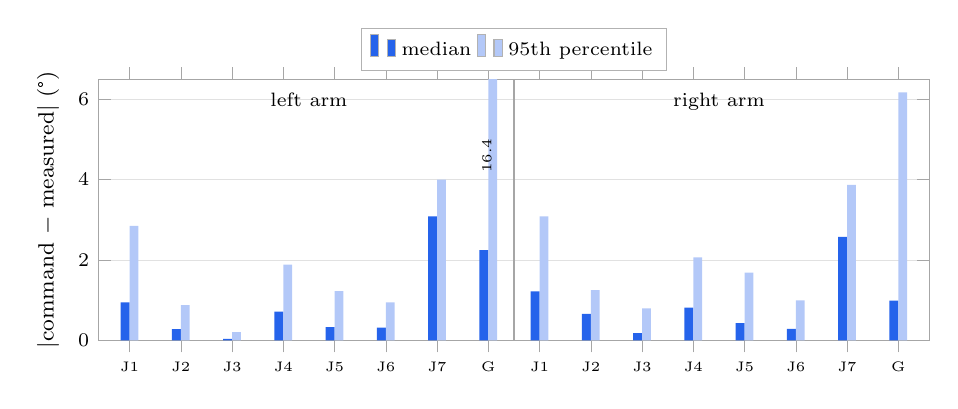
\begin{tikzpicture}
\begin{axis}[width=\columnwidth, height=4.9cm, ybar=0pt, bar width=3.2pt, ymin=0, ymax=6.5,
  xtick={1,...,16}, xticklabels={J1,J2,J3,J4,J5,J6,J7,G,J1,J2,J3,J4,J5,J6,J7,G},
  x tick label style={font=\tiny}, ylabel={$|$command $-$ measured$|$ (\textdegree)},
  ymajorgrids, legend style={at={(0.5,1.03)}, anchor=south, legend columns=2}, legend cell align=left, enlarge x limits=0.04]
\addplot[fill=cA, draw=none] coordinates {(1,0.95)(2,0.28)(3,0.04)(4,0.72)(5,0.33)(6,0.32)(7,3.09)(8,2.25)
  (9,1.22)(10,0.66)(11,0.18)(12,0.82)(13,0.43)(14,0.29)(15,2.58)(16,0.99)}; \addlegendentry{median}
\addplot[fill=cA!35, draw=none] coordinates {(1,2.85)(2,0.88)(3,0.21)(4,1.89)(5,1.23)(6,0.95)(7,4.00)(8,6.5)
  (9,3.09)(10,1.25)(11,0.80)(12,2.07)(13,1.69)(14,1.00)(15,3.87)(16,6.17)}; \addlegendentry{95th percentile}
\draw[gray!70] (axis cs:8.5,0) -- (axis cs:8.5,6.5);
\node[font=\scriptsize, anchor=north] at (axis cs:4.5,6.4) {left arm};
\node[font=\scriptsize, anchor=north] at (axis cs:12.5,6.4) {right arm};
\node[font=\tiny, anchor=south, rotate=90] at (axis cs:8.25,4.6) {16.4};
\end{axis}
\end{tikzpicture}
\caption{Tracking error per joint over the 30 demonstrations (24{,}412 frames): command sent to the follower vs its
measured position. G: gripper (left 95th percentile clipped, 16.4\textdegree, while squeezing an object).}
\label{fig:tracking}
\end{figure}

\subsection{Infrastructure fixes that mattered}
Two failures would have silently corrupted a data session. In the virtualised setup, a leader's serial port could be
opened once after plugging; every later open found no servo. Resetting the leaders' USB link before each open fixed it
(3/3 consecutive sessions opened, against 1/2 without). The top-view camera delivers about 11\,fps in the virtual
machine whatever the format; the recorder stores the latest frame at 30\,fps, so the dataset stays synchronous with the
joints and the policy sees the same duplicated-frame pattern at inference. The temperature guard caught the joint~3
overheat of \S\ref{sec:calib} before damage; with measured limits, no run has hit the guard since.

\subsection{Operators get faster}
Episodes got shorter as operators learned the task (Fig.~\ref{fig:episodes}): from 27.3\,s on average over the first ten
to 25.4\,s over the last ten (median 26.6\,s overall), with fewer hesitations---the long outliers are recovered grasps.
Faster demonstrations are not only cheaper: consistent, decisive demonstrations are easier to imitate
\citep{mandlekar2021matters}, which argues for a short warm-up session before recording a dataset.

\begin{figure}[t]
\centering
\begin{tikzpicture}
\begin{axis}[width=\columnwidth, height=4.4cm, xmin=-1, xmax=30, ymin=15, ymax=41,
  xlabel={episode}, ylabel={duration (s)}, ymajorgrids, legend style={at={(0.5,1.03)}, anchor=south, legend columns=2}, legend cell align=left]
\addplot[only marks, mark=*, mark size=1.4pt, cA!60] table[x=ep,y=dur] {data/episodes.dat}; \addlegendentry{episode}
\addplot[thick, cB] table[x=ep,y=roll] {data/episodes.dat}; \addlegendentry{mean of last 8}
\end{axis}
\end{tikzpicture}
\caption{Duration of the 30 demonstrations in recording order.}
\label{fig:episodes}
\end{figure}

\subsection{Policy success: decomposition wins}
Table~\ref{tab:success} and Fig.~\ref{fig:success} compare the policies trained on all 30 episodes. Chaining the four
per-skill ACT policies completes the task in \prov{17/20} trials, against \prov{7/20} for one ACT trained on whole
demonstrations and \prov{14/20} for $\pi_{0.5}$ with egocentric co-training (\prov{11/20} without). Each skill alone is
reliable (Table~\ref{tab:skills}): locate and release never failed, grasp is the weakest link, and the chain's success
is the product of its parts, so errors do not compound beyond it. With the same data, decomposition beats a
pretrained VLA. The per-skill policies never have to infer the phase of the task from pixels; the whole-task ACT
mostly fails by mixing phases, closing the gripper before reaching the tea bag or hesitating between objects.
$\pi_{0.5}$ copes better with placement but drops the tea bag at insertion. Egocentric co-training still helps the VLA
(\prov{+15} points).

\begin{table}[t]
\centering\small
\caption{Grasp-and-insert success over 20 trials per policy (30 teleoperated episodes), with 95\% Wilson intervals,
and the main failure mode.\provtag}
\label{tab:success}
\setlength{\tabcolsep}{3pt}
\begin{tabular}{@{}llrl@{}}
\toprule
Policy & Data & Success & Main failure\\
\midrule
ACT, whole task & teleop & \prov{7/20} {\scriptsize\prov{[18,57]}} & \prov{phases mixed}\\
$\pi_{0.5}$ & teleop & \prov{11/20} {\scriptsize\prov{[34,74]}} & \prov{dropped at insert}\\
$\pi_{0.5}$ & + ego & \prov{14/20} {\scriptsize\prov{[48,85]}} & \prov{dropped at insert}\\
ACT per skill & teleop & \prov{\textbf{17/20}} {\scriptsize\prov{[64,95]}} & \prov{grasp slip}\\
\bottomrule
\end{tabular}
\end{table}

\begin{table}[t]
\centering\small
\caption{Per-skill ACT policies, each evaluated alone from its own start state (20 trials), and chained.\provtag}
\label{tab:skills}
\begin{tabular}{@{}lrr@{}}
\toprule
Skill & Segments & Success\\
\midrule
\code{locate\_object} & 30 & \prov{20/20}\\
\code{grasp\_object} & 30 & \prov{18/20}\\
\code{move\_to\_location} & 30 & \prov{19/20}\\
\code{release\_object} & 30 & \prov{20/20}\\
\midrule
Chained & & \prov{17/20}\\
\bottomrule
\end{tabular}
\end{table}

\begin{figure}[t]
\centering
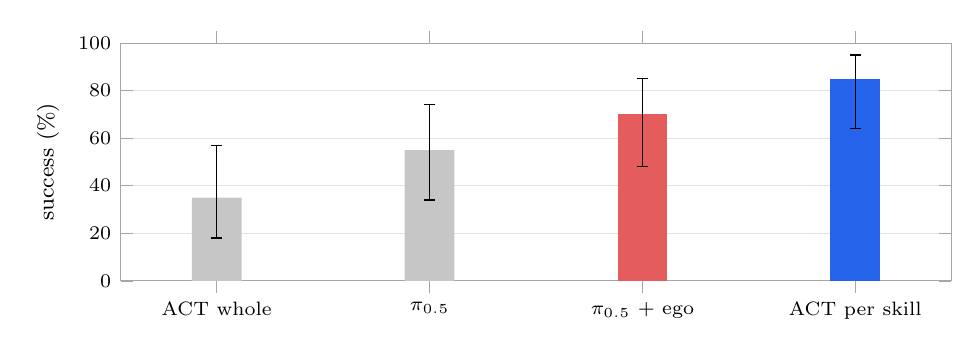
\begin{tikzpicture}
\begin{axis}[width=\columnwidth, height=4.6cm, ybar, bar width=18pt, bar shift=0pt, ymin=0, ymax=100,
  symbolic x coords={act,pi,piego,skill}, xtick={act,pi,piego,skill},
  xticklabels={ACT whole, $\pi_{0.5}$, $\pi_{0.5}$ + ego, ACT per skill}, enlarge x limits=0.15,
  ylabel={success (\%)}, ymajorgrids, error bars/y dir=both, error bars/y explicit]
\addplot[fill=gray!45, draw=none] coordinates {(act,35) += (0,22) -= (0,17) (pi,55) += (0,19) -= (0,21)};
\addplot[fill=cB!75, draw=none] coordinates {(piego,70) += (0,15) -= (0,22)};
\addplot[fill=cA, draw=none] coordinates {(skill,85) += (0,10) -= (0,21)};
\end{axis}
\end{tikzpicture}
\caption{Grasp-and-insert success with 30 teleoperated episodes (20 trials each, 95\% Wilson intervals).\provtag}
\label{fig:success}
\end{figure}

\subsection{Decomposition makes every episode count}\label{sec:res-scaling}
Fig.~\ref{fig:scaling} trains each policy on the first 10, 20 and 30 episodes. The horizontal reading gives two
discounts. Egocentric video lets $\pi_{0.5}$ reach with \prov{20} robot episodes what teleoperation alone reaches with
30, \prov{a third} fewer, close to the discount $\delta=0.4$ the bidder applies to $E_0$ when a gap matches an open
egocentric dataset (\S\ref{sec:bids}). Decomposition is the larger lever: the per-skill chain reaches the same success
with \prov{10} episodes, a third of the data, and its skills are reused by every plan that binds them, so their data is
paid for once.

\begin{figure}[t]
\centering
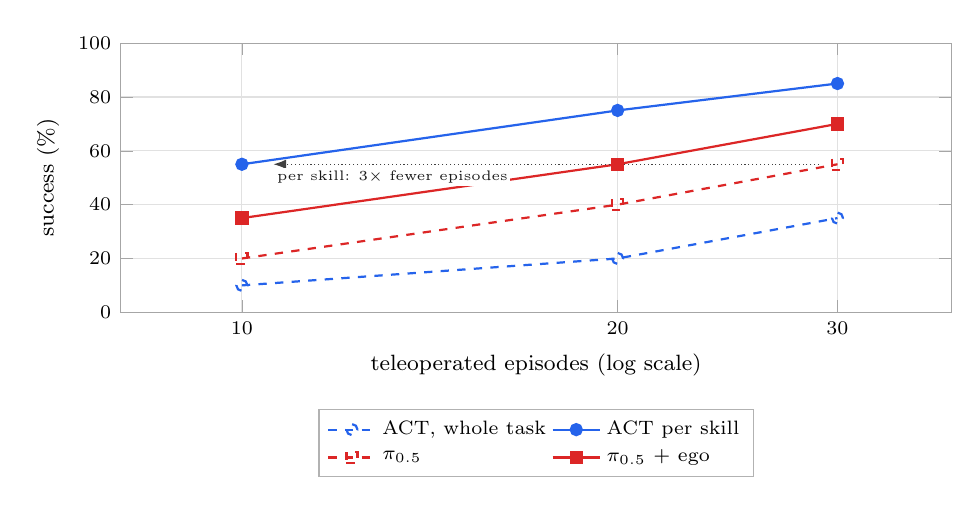
\begin{tikzpicture}
\begin{axis}[width=\columnwidth, height=5.0cm, xmode=log, log basis x=10, xmin=8, xmax=37, ymin=0, ymax=100,
  xtick={10,20,30}, xticklabels={10,20,30}, xlabel={teleoperated episodes (log scale)},
  ylabel={success (\%)}, grid=major, legend style={at={(0.5,-0.36)}, anchor=north, legend columns=2},
  legend cell align=left]
\addplot[cA, thick, dashed, mark=o] coordinates {(10,10) (20,20) (30,35)}; \addlegendentry{ACT, whole task}
\addplot[cA, thick, mark=*] coordinates {(10,55) (20,75) (30,85)}; \addlegendentry{ACT per skill}
\addplot[cB, thick, dashed, mark=square] coordinates {(10,20) (20,40) (30,55)}; \addlegendentry{$\pi_{0.5}$}
\addplot[cB, thick, mark=square*] coordinates {(10,35) (20,55) (30,70)}; \addlegendentry{$\pi_{0.5}$ + ego}
\draw[gray!50!black, densely dotted, -{Latex[length=1.6mm]}] (axis cs:29,55) -- (axis cs:10.6,55);
\node[font=\tiny, gray!20!black, anchor=north, fill=white, inner sep=1pt] at (axis cs:13.2,53.8) {per skill: 3$\times$ fewer episodes};
\end{axis}
\end{tikzpicture}
\caption{Data scaling: success against the number of teleoperated episodes (20 trials per point).\provtag}
\label{fig:scaling}
\end{figure}

\subsection{The crop is worth a dataset}
Training the per-skill policies on the uncropped top view and evaluating with the laptop moved and a person walking
behind the table drops chained success to \prov{45\%}; with the fixed crop it stays at \prov{80\%} (\prov{85\%} with an
undisturbed scene,
Table~\ref{tab:crop}). The distractors that a crop removes are exactly those that change between recording and
deployment, which is why we fixed the crop in the camera contract and re-encoded the old episodes instead of starting
a new dataset.

\begin{table}[t]
\centering\small
\caption{Effect of the top-view crop on the chained per-skill ACT policies (20 trials).\provtag}
\label{tab:crop}
\begin{tabular}{@{}lrr@{}}
\toprule
Scene at test time & Uncropped & Cropped\\
\midrule
As recorded & \prov{80\%} & \prov{85\%}\\
Laptop moved, person behind & \prov{45\%} & \prov{80\%}\\
\bottomrule
\end{tabular}
\end{table}

\subsection{From sentence to cup}
End to end, the request ``make me a cup of tea'' compiles to a valid plan on every run; the first steps bind to the
four newly trained skills and the pour to the scripted skill. Over \prov{10} full runs with the per-skill ACT chain,
\prov{9} complete locate, grasp, move and release and the handover, and \prov{8} pour within \prov{$\pm$5\,g} of the
requested mass. The handover
itself never failed: torque stays on through the switch, so the held objects do not move (Table~\ref{tab:e2e}).

\begin{table}[t]
\centering\small
\caption{End-to-end runs of ``make me a cup of tea'' (per-skill ACT, scripted pour).\provtag}
\label{tab:e2e}
\begin{tabular}{@{}lr@{}}
\toprule
Stage & Succeeded\\
\midrule
Plan compiled and valid & \prov{10/10}\\
Learned skills, chained & \prov{9/10}\\
Handover, torque kept on & \prov{9/9}\\
Pour within $\pm$5\,g (scripted) & \prov{8/9}\\
\midrule
Full request & \prov{8/10}\\
\bottomrule
\end{tabular}
\end{table}

% ===========================================================================
\section{Discussion}
\textbf{A checker substitutes for scale.} With two rounds of simulator feedback, planners roughly three times faster than
the largest reach the same final validity. For an interactive store this is the right trade: the checker is cheap and
exact, the model slow and approximate.

\textbf{The data gap is the dexterity gap---and egocentric video narrows it.} The motions compiled plans miss have
almost no robot demonstrations and are matched to human video instead. Our robot experiments turn that observation into
a lever: co-training on human video lets a VLA reach the same success with markedly fewer teleoperated episodes, so the
store can price, and buy, the missing skills more cheaply than a robot-only data market would.

\textbf{Decomposition beats pretraining at small data.} With 30 episodes, four small ACT policies, one per atomic
skill, outperform both a whole-task ACT and a fine-tuned $\pi_{0.5}$. The store's granularity is also the right
learning granularity: the skills the compiler composes are short, single-phase behaviours that action chunking learns
from a few dozen segments, they run without a GPU, and once trained they serve every plan that binds them. $\pi_{0.5}$
remains the stronger whole-task policy and gains most from egocentric video; we expect it to take over when a skill
needs language or wider generalisation.

\textbf{Safety is a property of the pipeline.} Because the compiler can be wrong, installation and dispatch re-run the
simulator rather than trusting a stored verdict, a queued plan cannot be edited, and an operator stop never sends the arm
home. The same principle runs down to the motors: torque is enabled only after a read-only preflight and a typed
\code{GO}, limits are measured rather than assumed, and a learned policy runs inside the exact loop that a human
teleoperates through. None of these gates depend on the model, or the operator, behaving well.

\textbf{Train and deploy on the same pixels.} Declaring each camera once, with its rotation, crop and zoom, and reading
that declaration in both the recorder and the runner removed a whole class of silent deployment failures. Changing the
contract later is possible, but only by rewriting the dataset with it.

\textbf{From valid to certified.} A store should publish, per skill and per robot, a measured success rate with a
confidence interval; with 20 trials, 18/20 is 90\% with a Wilson interval of 70--97\%. Validity is the necessary first
gate; measured success is the product.

\section{Limitations}
\textbf{Valid is not successful.} The simulator checks what the catalog declares; a plan it accepts can still fail on
hardware. \textbf{The requests are not a held-out test set.} Prompts and start-state assumptions were revised while
inspecting failures on these same requests. \textbf{Small samples.} Thirteen requests and 3 runs per planner, and 20
trials per policy, give wide intervals; differences of a few points are not significant. \textbf{One task, one
robot.} Policy results cover one bimanual task on one OpenArm in one room; the egocentric discount may differ for
motions whose human and robot embodiments diverge more (in-hand rotation, tool use with fingers). \textbf{Segmentation is
semi-automatic.} Skill boundaries come from gripper events and were checked by hand. \textbf{Retargeting
is approximate.} Human wrist poses are mapped to a 7-DoF arm with a parallel gripper; finger-level detail is lost.
\textbf{The market is simulated.} Bids come from our own compilations; real demand will differ. \textbf{Scheduling
ignores gaps' timing}, since gaps have no duration until they are trained.

\section{Conclusion}
Separating \emph{acting out} a request from \emph{binding} it to products, and letting a declarative simulator veto and
explain, turns language models into usable compilers for a skill store. Closing the loop on a real bimanual robot turns
the store's gaps into skills: a safety-gated teleoperation stack with measured limits and a frozen camera contract
produces clean demonstrations, and splitting them into the catalog's atomic skills, one ACT policy each, yields a chain
that beats a fine-tuned VLA trained on the same 30 episodes and hands over to a scripted pour. Human video is not only where the compiler finds candidate data for missing
skills; it is what makes those skills cheap enough to buy. Next steps are canonicalising gap names into a motion
taxonomy, training the most demanded gaps from egocentric data first, and publishing measured success rates per skill.

% ===========================================================================
\small
\begin{thebibliography}{99}\setlength{\itemsep}{0.1em}
\bibitem[Ahn et~al.(2022)]{ahn2022saycan} M.~Ahn, A.~Brohan, N.~Brown, et~al. Do as I can, not as I say: Grounding language in robotic affordances. \emph{arXiv preprint arXiv:2204.01691}, 2022.
\bibitem[Black et~al.(2024)]{black2024pi0} K.~Black, N.~Brown, D.~Driess, et~al. $\pi_0$: A vision-language-action flow model for general robot control. \emph{arXiv preprint arXiv:2410.24164}, 2024.
\bibitem[Brohan et~al.(2023)]{brohan2023rt2} A.~Brohan, N.~Brown, J.~Carbajal, et~al. RT-2: Vision-language-action models transfer web knowledge to robotic control. In \emph{CoRL}, 2023.
\bibitem[Cadene et~al.(2024)]{cadene2024lerobot} R.~Cadene, S.~Alibert, A.~Soare, et~al. LeRobot: State-of-the-art machine learning for real-world robotics in PyTorch. \url{https://github.com/huggingface/lerobot}, 2024.
\bibitem[Chi et~al.(2023)]{chi2023diffusion} C.~Chi, S.~Feng, Y.~Du, Z.~Xu, E.~Cousineau, B.~Burchfiel, and S.~Song. Diffusion Policy: Visuomotor policy learning via action diffusion. In \emph{RSS}, 2023.
\bibitem[Damen et~al.(2022)]{damen2022epic} D.~Damen, H.~Doughty, G.~M. Farinella, et~al. Rescaling egocentric vision: Collection, pipeline and challenges for EPIC-KITCHENS-100. \emph{IJCV}, 130:33--55, 2022.
\bibitem[Enactic(2025)]{enactic2025openarm} Enactic. OpenArm: An open-source robot arm for physical AI research. \url{https://github.com/enactic/openarm}, 2025.
\bibitem[Fikes and Nilsson(1971)]{fikes1971strips} R.~E. Fikes and N.~J. Nilsson. STRIPS: A new approach to the application of theorem proving to problem solving. \emph{Artificial Intelligence}, 2(3--4):189--208, 1971.
\bibitem[Fu et~al.(2024)]{fu2024mobilealoha} Z.~Fu, T.~Z. Zhao, and C.~Finn. Mobile ALOHA: Learning bimanual mobile manipulation with low-cost whole-body teleoperation. In \emph{CoRL}, 2024.
\bibitem[Garrett et~al.(2021)]{garrett2021tamp} C.~R. Garrett, R.~Chitnis, R.~Holladay, B.~Kim, T.~Silver, L.~P. Kaelbling, and T.~Lozano-Pérez. Integrated task and motion planning. \emph{Annual Review of Control, Robotics, and Autonomous Systems}, 4:265--293, 2021.
\bibitem[Grauman et~al.(2022)]{grauman2022ego4d} K.~Grauman, A.~Westbury, E.~Byrne, et~al. Ego4D: Around the world in 3,000 hours of egocentric video. In \emph{CVPR}, 2022.
\bibitem[Grauman et~al.(2024)]{grauman2024egoexo4d} K.~Grauman, A.~Westbury, L.~Torresani, et~al. Ego-Exo4D: Understanding skilled human activity from first- and third-person perspectives. In \emph{CVPR}, 2024.
\bibitem[Hogan(1985)]{hogan1985impedance} N.~Hogan. Impedance control: An approach to manipulation. \emph{ASME Journal of Dynamic Systems, Measurement, and Control}, 107(1):1--24, 1985.
\bibitem[Hoque et~al.(2025)]{hoque2025egodex} R.~Hoque, P.~Huang, D.~J. Yoon, M.~Sivapurapu, and J.~Zhang. EgoDex: Learning dexterous manipulation from large-scale egocentric video. \emph{arXiv preprint arXiv:2505.11709}, 2025.
\bibitem[Huang et~al.(2022a)]{huang2022zeroshot} W.~Huang, P.~Abbeel, D.~Pathak, and I.~Mordatch. Language models as zero-shot planners: Extracting actionable knowledge for embodied agents. In \emph{ICML}, 2022.
\bibitem[Huang et~al.(2022b)]{huang2022innermonologue} W.~Huang, F.~Xia, T.~Xiao, et~al. Inner monologue: Embodied reasoning through planning with language models. In \emph{CoRL}, 2022.
\bibitem[Huang et~al.(2023)]{huang2023voxposer} W.~Huang, C.~Wang, R.~Zhang, Y.~Li, J.~Wu, and L.~Fei-Fei. VoxPoser: Composable 3D value maps for robotic manipulation with language models. In \emph{CoRL}, 2023.
\bibitem[{ISO}(2016)]{iso15066} ISO/TS 15066:2016. Robots and robotic devices---Collaborative robots. International Organization for Standardization, 2016.
\bibitem[Kambhampati et~al.(2024)]{kambhampati2024llmmodulo} S.~Kambhampati, K.~Valmeekam, L.~Guan, et~al. Position: LLMs can't plan, but can help planning in LLM-Modulo frameworks. In \emph{ICML}, 2024.
\bibitem[Kareer et~al.(2024)]{kareer2024egomimic} S.~Kareer, D.~Patel, R.~Punamiya, P.~Mathur, S.~Cheng, C.~Wang, J.~Hoffman, and D.~Xu. EgoMimic: Scaling imitation learning via egocentric video. \emph{arXiv preprint arXiv:2410.24221}, 2024.
\bibitem[Khazatsky et~al.(2024)]{khazatsky2024droid} A.~Khazatsky, K.~Pertsch, S.~Nair, et~al. DROID: A large-scale in-the-wild robot manipulation dataset. In \emph{RSS}, 2024.
\bibitem[Kim et~al.(2024)]{kim2024openvla} M.~J. Kim, K.~Pertsch, S.~Karamcheti, et~al. OpenVLA: An open-source vision-language-action model. In \emph{CoRL}, 2024.
\bibitem[Konidaris and Barto(2009)]{konidaris2009chaining} G.~Konidaris and A.~Barto. Skill discovery in continuous reinforcement learning domains using skill chaining. In \emph{NeurIPS}, 2009.
\bibitem[Kostrikov et~al.(2021)]{kostrikov2021drq} I.~Kostrikov, D.~Yarats, and R.~Fergus. Image augmentation is all you need: Regularizing deep reinforcement learning from pixels. In \emph{ICLR}, 2021.
\bibitem[Laskin et~al.(2020)]{laskin2020rad} M.~Laskin, K.~Lee, A.~Stooke, L.~Pinto, P.~Abbeel, and A.~Srinivas. Reinforcement learning with augmented data. In \emph{NeurIPS}, 2020.
\bibitem[Liang et~al.(2023)]{liang2023cap} J.~Liang, W.~Huang, F.~Xia, et~al. Code as policies: Language model programs for embodied control. In \emph{ICRA}, 2023.
\bibitem[Lin et~al.(2023)]{lin2023text2motion} K.~Lin, C.~Agia, T.~Migimatsu, M.~Pavone, and J.~Bohg. Text2Motion: From natural language instructions to feasible plans. \emph{Autonomous Robots}, 47:1345--1365, 2023.
\bibitem[Lin et~al.(2025)]{lin2025scaling} F.~Lin, Y.~Hu, P.~Sheng, C.~Wen, J.~You, and Y.~Gao. Data scaling laws in imitation learning for robotic manipulation. In \emph{ICLR}, 2025.
\bibitem[Liu et~al.(2023)]{liu2023llmp} B.~Liu, Y.~Jiang, X.~Zhang, Q.~Liu, S.~Zhang, J.~Biswas, and P.~Stone. LLM+P: Empowering large language models with optimal planning proficiency. \emph{arXiv preprint arXiv:2304.11477}, 2023.
\bibitem[Mandlekar et~al.(2021)]{mandlekar2021matters} A.~Mandlekar, D.~Xu, J.~Wong, et~al. What matters in learning from offline human demonstrations for robot manipulation. In \emph{CoRL}, 2021.
\bibitem[McDermott et~al.(1998)]{mcdermott1998pddl} D.~McDermott, M.~Ghallab, A.~Howe, C.~Knoblock, A.~Ram, M.~Veloso, D.~Weld, and D.~Wilkins. PDDL---the planning domain definition language. Technical Report CVC TR-98-003, Yale Center for Computational Vision and Control, 1998.
\bibitem[Nair et~al.(2022)]{nair2022r3m} S.~Nair, A.~Rajeswaran, V.~Kumar, C.~Finn, and A.~Gupta. R3M: A universal visual representation for robot manipulation. In \emph{CoRL}, 2022.
\bibitem[NVIDIA(2025)]{nvidia2025groot} NVIDIA, J.~Bjorck, F.~Castañeda, et~al. GR00T N1: An open foundation model for generalist humanoid robots. \emph{arXiv preprint arXiv:2503.14734}, 2025.
\bibitem[Octo Model Team(2024)]{octo2024} Octo Model Team, D.~Ghosh, H.~Walke, K.~Pertsch, et~al. Octo: An open-source generalist robot policy. In \emph{RSS}, 2024.
\bibitem[Open X-Embodiment(2024)]{oxe2024} Open X-Embodiment Collaboration. Open X-Embodiment: Robotic learning datasets and RT-X models. In \emph{ICRA}, 2024.
\bibitem[Physical Intelligence(2025)]{pi2025pi05} Physical Intelligence, K.~Black, N.~Brown, et~al. $\pi_{0.5}$: A vision-language-action model with open-world generalization. \emph{arXiv preprint arXiv:2504.16054}, 2025.
\bibitem[Qiu et~al.(2025)]{qiu2025humanoid} R.-Z. Qiu, S.~Yang, X.~Cheng, et~al. Humanoid policy $\sim$ human policy. \emph{arXiv preprint arXiv:2503.13441}, 2025.
\bibitem[Siciliano et~al.(2009)]{siciliano2009robotics} B.~Siciliano, L.~Sciavicco, L.~Villani, and G.~Oriolo. \emph{Robotics: Modelling, Planning and Control}. Springer, 2009.
\bibitem[Singh et~al.(2023)]{singh2023progprompt} I.~Singh, V.~Blukis, A.~Mousavian, et~al. ProgPrompt: Generating situated robot task plans using large language models. In \emph{ICRA}, 2023.
\bibitem[Sutton et~al.(1999)]{sutton1999options} R.~S. Sutton, D.~Precup, and S.~Singh. Between MDPs and semi-MDPs: A framework for temporal abstraction in reinforcement learning. \emph{Artificial Intelligence}, 112(1--2):181--211, 1999.
\bibitem[Valmeekam et~al.(2023)]{valmeekam2023planbench} K.~Valmeekam, M.~Marquez, A.~Olmo, S.~Sreedharan, and S.~Kambhampati. PlanBench: An extensible benchmark for evaluating large language models on planning and reasoning about change. In \emph{NeurIPS Datasets and Benchmarks}, 2023.
\bibitem[Wang et~al.(2023)]{wang2023mimicplay} C.~Wang, L.~Fan, J.~Sun, R.~Zhang, L.~Fei-Fei, D.~Xu, Y.~Zhu, and A.~Anandkumar. MimicPlay: Long-horizon imitation learning by watching human play. In \emph{CoRL}, 2023.
\bibitem[Wilson(1927)]{wilson1927} E.~B. Wilson. Probable inference, the law of succession, and statistical inference. \emph{JASA}, 22(158):209--212, 1927.
\bibitem[Wu et~al.(2024)]{wu2024gello} P.~Wu, Y.~Shentu, Z.~Yi, X.~Lin, and P.~Abbeel. GELLO: A general, low-cost, and intuitive teleoperation framework for robot manipulators. In \emph{IROS}, 2024.
\bibitem[Zhao et~al.(2023)]{zhao2023aloha} T.~Z. Zhao, V.~Kumar, S.~Levine, and C.~Finn. Learning fine-grained bimanual manipulation with low-cost hardware. In \emph{RSS}, 2023.
\bibitem[Zhao et~al.(2024)]{zhao2024unleashed} T.~Z. Zhao, J.~Tompson, D.~Driess, et~al. ALOHA Unleashed: A simple recipe for robot dexterity. In \emph{CoRL}, 2024.
\end{thebibliography}
\normalsize

% ===========================================================================
\appendix
\section{Requests and object kinds}\label{app:kinds}
\textbf{Unfamiliar requests (N).} ``You have a paint bucket and brush. draw an image on the table''; ``build a small
sandcastle on the tray with the bucket and shovel''; ``do a simple card trick with the deck on the table''; ``water the
two plants on the shelf''; ``write my name on the whiteboard with the marker''; ``make me a jam sandwich''; ``put the
flowers in the vase and add water''; ``feed the cat: open the tin and put the food in her bowl''. \textbf{Demo requests
(D).} ``make me a pina colada''; ``pour me a glass of juice''; ``mix me a smoothie''; ``wipe my table clean after
dinner''; ``clear the table and put the bottles away''.

\textbf{Object kinds.} \code{bottle}: a rigid bottle, carton or jug of liquid, held upright; \code{glass}: a drinking
glass, cup or mug; \code{shaker}: a cocktail shaker; \code{scoop}: a measuring scoop with a handle; \code{cloth}:
something soft and deformable; \code{item}: any other rigid, hand-sized loose thing; \code{fixed}: something that is
not picked up (a table, a shelf, an appliance); \code{substance}: a material inside something else (paint, water, sand).

\section{Simulator checks}\label{app:checks}
\begin{table}[h]
\centering\small
\caption{Every check the simulator runs; \emph{adv.}: advisory, returned to the binder but not blocking installation.}
\begin{tabular}{@{}p{0.33\columnwidth}p{0.6\columnwidth}@{}}
\toprule
Check & Raised when\\
\midrule
Unmet precondition & a step needs a fact, on its hand, that no earlier step or gap established\\
Wrong object kind & the skill's \code{acts\_on} does not include the kind of its target\\
Wrong pour direction & the held object is the target, or is an empty glass or shaker\\
Embodiment mismatch & the skill needs a body (torso, base) the robot lacks\\
Unknown skill & a step names a skill outside the catalog (prevented by the enum)\\
Empty plan & the binding contains no executable step\\
Ends holding (adv.) & a hand still holds or has located something at the end\\
Pointless move (adv.) & an object is picked up and set back where it was, unused\\
\bottomrule
\end{tabular}
\end{table}
\textbf{Repair hints.} Each issue returns with a catalog-derived hint: the skills that establish a missing fact, the
containers holding something, or the skill a duplicate gap restates.

\section{Robot configuration}\label{app:robot}
\begin{table}[h]
\centering\small
\caption{Robot, recording and training parameters.}
\footnotesize\begin{tabular}{@{}lp{0.6\columnwidth}@{}}
\toprule
Parameter & Value\\
\midrule
Arms & 2 $\times$ OpenArm v10, 7 DoF + gripper\\
Motors & Damiao DM8009 / DM4340 / DM4310\\
Bus & 2 $\times$ CAN-FD, 1 / 5\,Mbps, sample point 0.75\\
Leaders & 2 $\times$ OpenArm Mini (Feetech)\\
Control / dataset rate & 60\,Hz / 30\,fps\\
Cameras & D455 (front), USB top view (back), 640$\times$480\\
Camera preprocessing & front: rot.\ 180\textdegree, zoom 1.1$\times$; back: crop 512$\times$384 @ (16,40)\\
State / action & 16-D joint positions (deg) / 16-D commands\\
Dataset & 30 episodes, 24{,}412 frames, H.264, LeRobot v3\\
ACT & one per skill (4), chunk 100, ResNet-18, \prov{50k} steps, batch 8\\
$\pi_{0.5}$ & base checkpoint, \prov{30k} steps, batch \prov{32}\\
Egocentric mix & \prov{25\%} of each batch, robot-only normalisation\\
\bottomrule
\end{tabular}
\end{table}

\end{document}
